\chapter{Analysis and Design}
\label{chap:proposed.work}

\section{Bayes by Backprop}

Bayes by Backprop \cite{Blundell2015a} is a variational inference scheme for learning the posterior distribution on the weights of a neural network.
The posterior distribution on parameters of the network $\theta \in \mathbb{R}^d$, $q(\theta)$ is typically taken to be a Gaussian with mean parameter $\mu\in \mathbb{R}^d$ and standard deviation parameter $\sigma\in \mathbb{R}^d$, denoted $\mathcal{N}(\theta|\mu,\sigma)$ and it's a diagonal covariance matrix. Where $d$ is the dimensionality of the parameters of the network (usually refers to scale of millions).
Let $\log p(y|\theta, x)$ be the log-likelihood of the neural network, then the network is trained by minimising the variational free energy, where $p(\theta)$ is a prior on the parameters:

\begin{align}
	\label{eq:elbo}
	\mathcal{L}(\theta) &=
	\mathbb{E}_{q(\theta)}\left[\log \frac{q(\theta)}{p(y|\theta, x)p(\theta)}\right],
\end{align}

The \textbf{algorithm \ref{alg:bbb}} shows the Bayes by Backprop Monte Carlo procedure for minimising the above equation with respect to the mean and standard deviation parameters of the posterior $q(\theta)$.

Minimising the variational free energy equation is equivalent to maximising the log-likelihood $\log p(y|\theta, x)$ subject to a KL complexity term in the parameters of the network that acts as a regulariser:

\begin{align}
	\label{eq:klelbo}
	\mathcal{L}(\theta) &=
	- \mathbb{E}_{q(\theta)}\left[\log p(y|\theta, x) \right]
	+ \kl{q(\theta)}{p(\theta)}.
\end{align}

Gaussian process in a case with zero mean prior, the KL term acts as a form of weight decay on the mean parameters, where the rate of weight decay is automatically tuned by the standard deviation parameters of the prior and posterior.

\begin{algorithm}[ht]
	\caption{Bayes by Backprop}
	\label{alg:bbb}
	\begin{algorithmic}
		\STATE{Sample $\epsilon \sim \mathcal{N}(0, I)$, $\epsilon \in \mathbb{R}^d$.}
		\STATE{Set network parameters to $\theta = \mu + \sigma\epsilon$.}
		\STATE{Do forward propagation and backpropagation as normal.}
		\STATE{Let $g$ be the gradient with respect	\label{eq:elbo}
			\mathcal{L}(\theta) &=
			\mathbb{E}_{q(\theta)}\left[\log \frac{q(\theta)}{p(y|\theta, x)p(\theta)}\right], to $\theta$ from backpropagation.} 
		\STATE{Let $g^{KL}_\theta, g^{KL}_\mu, g^{KL}_\sigma$ be the gradients of $\log \mathcal{N}(\theta|\mu, \sigma) - \log p(\theta)$ with respect to $\theta$, $\mu$ and 
			$\sigma$ respectively.} 
		\STATE{Update $\mu$ according to the gradient $g + g^{KL}_\theta + g^{KL}_\mu$.} 
		\STATE{Update $\sigma$ according to the gradient $(g + g^{KL}_\theta) \epsilon + g^{KL}_\sigma$.}
	\end{algorithmic}
\end{algorithm}

The uncertainty afforded by Bayes by Backprop trained networks has been used successfully for training feed-forward NN models for supervised learning and also to help exploration to reinforcement learning agents \cite{Blundell2015a}, \cite{Lipton2016}, \cite{Houthooft2016}, but until now, BBB has not been applied to recurrent neural networks.

\section{Adoption of Bayes by Backprop to RNNs}
\label{sec:tbbbtt}

Applying Bayes by Backprop (BBB) to RNNs is illustrated in \textbf{Figure \ref{fig:lstmbbb}} where the weight matrices of the RNN are drawn from a distribution (learnt by BBB).
However, this direct application raises two questions: when to sample the parameters of the RNN, and how to weight the contribution of the KL regulariser of \eqref{eq:klelbo}.
To address these concerns in the adaptation of BBB to RNNs, Algorithm \ref{alg:rnnbbb} given where:

\begin{figure}
	\centering
	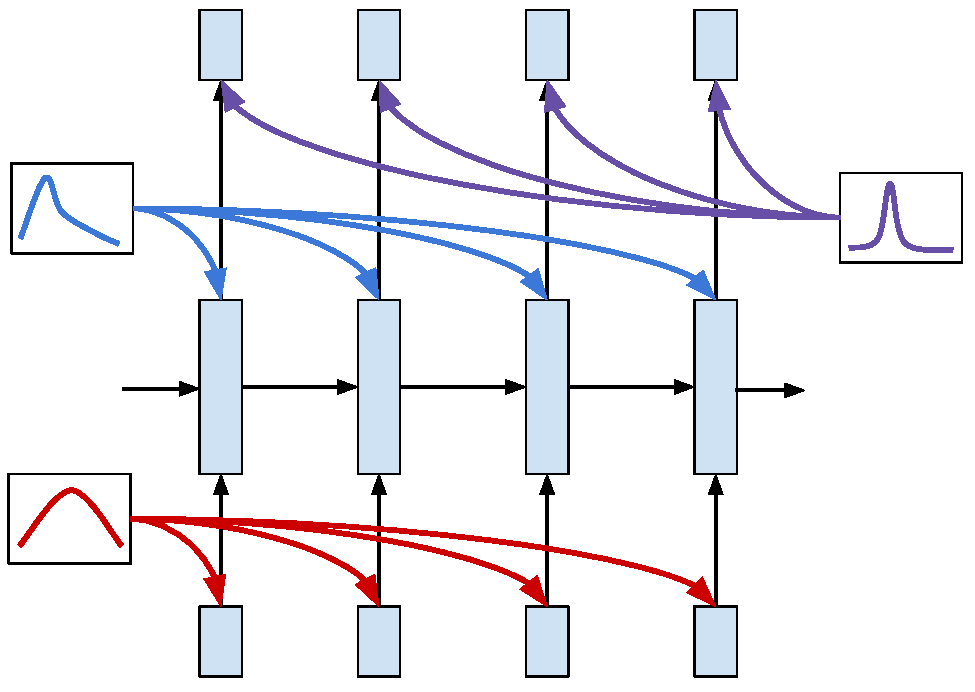
\includegraphics[width=\linewidth]{figs/LSTMBBB}
	\caption{Adoption of Bayes by Backprop (BBB) to an RNN.}
	\label{fig:lstmbbb}
\end{figure}

The variational free energy of \eqref{eq:klelbo} for an RNN on a sequence of length $T$ is:

\begin{align}
	\mathcal{L}(\theta) &=
	- \mathbb{E}_{q(\theta)}\left[\log p(y_{1:T}|\theta, x_{1:T}) \right]
	\nonumber \\
	&\phantom{=}
	+ \kl{q(\theta)}{p(\theta)},
	\label{eq:rnnelbo}
\end{align}

where $p(y_{1:T}|\theta, x_{1:T})$ is the likelihood of a sequence produced when the states of an unrolled RNN $F_T$ are fed into an appropriate probability distribution.
The parameters of the entire network are $\theta$.
Although the RNN is unrolled $T$ times, each weight is penalised just once by the KL term, rather than $T$ times.
Also clear from \eqref{eq:rnnelbo} is that when a Monte Carlo approximation is taken to the expectation, the parameters $\theta$ should be held fixed throughout the entire sequence.

Two complications arise to the above naive derivation in practice: firstly, sequences are often long enough and models sufficiently large, that unrolling the RNN for the whole sequence is prohibitive.
Secondly, to reduce variance in the gradients, more than one sequence is trained at a time.
Thus the typical regime for training RNNs involves training on mini-batches of truncated sequences.

Let $B$ be the number of mini-batches and $C$ the number of truncated sequences (``cuts''),
then we can write \eqref{eq:rnnelbo} as:
\begin{align}
	\mathcal{L}(\theta) &=
	- \mathbb{E}_{q(\theta)}\left[\log \prod_{b=1}^B \prod_{c=1}^{C} p(y^{(b,c)}|\theta, x^{(b,c)}) \right]
	\nonumber \\
	&\phantom{=}
	+ \kl{q(\theta)}{p(\theta)},
\end{align}
where the $(b,c)$ superscript denotes elements of $c$th truncated sequence in the $b$th minibatch.
Thus the free energy of mini-batch $b$ of a truncated sequence $c$ can be written as:
\begin{align}
	\mathcal{L}_{(b,c)}(\theta) &=
	- \mathbb{E}_{q(\theta)}\left[\log p(y^{(b,c)}|\theta, x^{(b,c)}, s^{(b,c)}_\text{prev}) \right]
	\nonumber \\
	&\phantom{=}
	+ w^{(b,c)}_\text{KL} \kl{q(\theta)}{p(\theta)},
	\label{eq:weightelbo}
\end{align}
where $w^{(b,c)}_\text{KL}$ distributes the responsibility of the KL cost among minibatches and truncated sequences (thus $\sum_{b=1}^B \sum_{c=1}^C w^{(b,c)}_\text{KL} = 1$), and $s^{(b,c)}_\text{prev}$ refers to the initial state of the RNN for the minibatch $x^{(b,c)}$.
In practice, we pick $w^{(b,c)}_\text{KL} = \frac{1}{C B}$ so that the KL penalty is equally distributed among all mini-batches and truncated sequences.
The truncated sequences in each subsequent mini-batches are picked in order, and so $s^{(b,c)}_\text{prev}$ is set to the last state of the RNN for $x^{(b,c-1)}$.

Finally, the question of when to sample weights follows naturally from taking a Monte Carlo approximations to \eqref{eq:weightelbo}: for each minibatch, sample a fresh set of parameters.

\begin{algorithm}[ht]
	\caption{Bayes by Backprop for RNNs}
	\label{alg:rnnbbb}
	\begin{algorithmic}
		\STATE{Sample $\epsilon \sim \mathcal{N}(0,I)$, $\epsilon \in \mathbb{R}^d$.}
		\STATE{Set network parameters to $\theta = \mu + \sigma\epsilon$.}
		\STATE{Sample a minibatch of truncated sequences $(x,y)$.}
		\STATE{Do forward propagation and backpropagation as normal on minibatch.}
		\STATE{Let $g$ be the gradient with respect to $\theta$ from backpropagation.}
		\STATE{Let $g^{KL}_\theta, g^{KL}_\mu, g^{KL}_\sigma$ be the gradients of $\log \mathcal{N}(\theta|\mu, \sigma) - \log p(\theta)$ w.r.t. $\theta$, $\mu$ and $\sigma$ respectively.}
		\STATE{Update $\mu$ according to the gradient $\frac{g + \frac{1}{C}g^{KL}_\theta}{B} + \frac{g^{KL}_\mu}{B C}$.}
		\STATE{Update $\sigma$ according to the gradient $\left(\frac{g + \frac{1}{C} g^{KL}_\theta}{B}\right) \epsilon + \frac{g^{KL}_\sigma}{B C}$.}
	\end{algorithmic}
\end{algorithm}

\section{Chapter Summary}